\documentclass[12pt, a4paper]{article}
\usepackage[UTF8]{ctex} % 支持中文
\usepackage{amsmath, amssymb, amsthm, bm}
\usepackage{geometry}
\usepackage{graphicx}
\usepackage{booktabs} % 更好的表格线
\usepackage{float} % 强制图片/表格位置
\usepackage{xcolor}
\usepackage{enumitem}
\usepackage{fancyhdr}
\usepackage{lastpage}
\usepackage{caption} % 修复 \captionof 问题
\usepackage[most]{tcolorbox} % 美化题目框
\usepackage[ruled,vlined,linesnumbered]{algorithm2e} % 专业算法排版
\usepackage{amssymb} % 需要此宏包来显示黑色方块 \blacksquare

% --- 页面设置 ---
\geometry{left=2.5cm, right=2.5cm, top=2.5cm, bottom=2.5cm, headheight=15pt}
\pagestyle{fancy}
\fancyhf{}
\fancyhead[L]{第35章 马尔可夫决策过程}
\fancyhead[R]{习题解答}
\fancyfoot[C]{第 \thepage 页 / 共 \pageref{LastPage} 页}
\renewcommand{\headrulewidth}{0.5pt}

% --- 颜色定义 ---
\definecolor{themecolor}{RGB}{0, 51, 102} % 深蓝色主题
\definecolor{boxback}{RGB}{245, 247, 250} % 浅灰蓝背景

% --- 自定义环境 ---
% 题目环境
\newtcolorbox{problem}[1][]{
	enhanced,
	colback=boxback,
	colframe=themecolor,
	fonttitle=\bfseries,
	title={#1},
	attach boxed title to top left={yshift*=-\tcboxedtitleheight/2, xshift=5mm},
	boxed title style={colback=themecolor},
	before skip=0.5cm,
	after skip=0.5cm
}

% 解答环境 【修改：去除了结尾的 \hrule】
\newenvironment{solution}{
	\par\vspace{0.2cm}\noindent\textbf{\color{themecolor} \textit{解：}}
}{
	\par\vspace{0.5cm} % 仅保留垂直间距，去除横线
}

% 证明环境重定义 【修改：去除了结尾的 \hrule】
\renewenvironment{proof}{
	\par\vspace{0.2cm}\noindent\textbf{\color{themecolor} \textit{证明：}}
}{
	\hfill $\blacksquare$ \par\vspace{0.5cm} % 仅保留垂直间距，去除横线
}

% --- 自定义命令 (保留您的定义) ---
\newcommand{\up}{\ensuremath{\uparrow}}
\newcommand{\down}{\ensuremath{\downarrow}}
\newcommand{\leftarrowcmd}{\ensuremath{\leftarrow}}
\newcommand{\rightarrowcmd}{\ensuremath{\rightarrow}}
\newcommand{\goal}{\ensuremath{\oplus}}
\newcommand{\trap}{\ensuremath{\text{陷阱}}}
\newcommand{\wall}{\ensuremath{\blacksquare}}

% 算法中文化的设置
\SetKwInput{KwIn}{输入}
\SetKwInput{KwOut}{输出}
\SetKwInput{KwParam}{参数}

\title{\textbf{\huge 第35章 马尔可夫决策过程\\ \large 习题参考答案}}
\author{}
\date{}

\begin{document}
	
	\maketitle
	\thispagestyle{empty}
	
	% ==========================================
	% 35.1
	% ==========================================
	\begin{problem}[习题 35.1]
		假设奖励属于有限集合 $R \in \mathcal{R}$，折扣因子 $\gamma < 1$，证明回报一定有界。
		
		\small{\textbf{提示：}利用以下关系：
			\[ G_t = \sum_{k=0}^{\infty} \gamma^k R_{t+k+1} \]
			\[ \sum_{k=0}^{\infty} \gamma^k = \frac{1}{1-\gamma}, \quad \gamma < 1 \]
		}
	\end{problem}
	
	\begin{proof}
		因为奖励属于有限集合，所以它是有界集。
		即存在 $M > 0$，使得对于任意 $r \in \mathcal{R}$，都有 $|r| \le M$。
		即 $\forall k \in \mathbb{N}, |R_{t+k+1}| \le M$。
		
		则回报 $G_t$ 的绝对值为：
		\begin{align*}
			|G_t| &= \left| \sum_{k=0}^{\infty} \gamma^k R_{t+k+1} \right| \\
			&\le \sum_{k=0}^{\infty} \gamma^k |R_{t+k+1}|\text{(三角不等式)} \\
			&\le M \sum_{k=0}^{\infty} \gamma^k \\
			&= \frac{M}{1-\gamma}
		\end{align*}
		因为 $\frac{M}{1-\gamma}$ 是有限常数，所以回报一定有界。
	\end{proof}
	
	% ==========================================
	% 35.2
	% ==========================================
	\clearpage
	\begin{problem}[习题 35.2]
		写出有限期MDP的一个轨迹上各个状态的回报的递归计算算法。
	\end{problem}
	
\begin{solution}
	设有限期一条轨迹为 $S_0, A_0, R_1, S_1, A_1, R_2, \dots, S_T$，其中 $T$ 是终止时刻。
	$\gamma$ 为折扣因子。
	对于 $t = 0, \dots, T-1$，
	\[ 
	G_t = R_{t+1} + \gamma R_{t+2} + \dots + \gamma^{T-t-1} R_T 
	= R_{t+1} + \gamma (R_{t+2} + \dots + \gamma^{T-t-2}R_T) 
	\]
	
	\textbf{得到递归关系式：}
	\[ G_t = R_{t+1} + \gamma G_{t+1} \]
	
	\vspace{1em}
	
	\begin{algorithm}[H]
		\renewcommand{\thealgocf}{} % <--- 添加这一行来隐藏算法编号
		\caption{计算回报的递归算法}
		\KwIn{有限期轨迹 $S_0, A_0, R_1, S_1, A_1, R_2, \dots, S_T$。}
		\KwOut{各时刻的回报 $G_0, G_1, \dots, G_{T-1}$。}
		\KwParam{折扣因子 $\gamma$。}
		
		\tcp{初始化终止时刻的回报}
		$G_T = 0$\;
		
		\tcp{从后向前逆序计算回报}
		\For{$t = T-1, T-2, \dots, 0$}{
			$G_t \leftarrow R_{t+1} + \gamma G_{t+1}$\;
			\tcp{记录当前时刻 $t$ 对应的回报 $G_t$}
		}
		\Return $\{G_t\}_{t=0}^{T-1}$\;
	\end{algorithm}
\end{solution}
	
	% ==========================================
	% 35.3
	% ==========================================
	\clearpage
	\begin{problem}[习题 35.3]
		例35.1的问题中，计算策略是 $\pi_1$ 和 $\pi_2$ 时的轨迹的回报和概率。
	\end{problem}
	
	\begin{solution}
		已知折扣因子 $\gamma = 0.9$。
		
		\textbf{(1) 当策略是 $\pi_2$ 时：}
		\begin{itemize}
			\item[] \textbf{轨迹 $t_1$:} $(1,1) \to (1,2) \to (1,3) \to (2,3) \to (3,3) \to (4,3)$
			\item[] \textbf{轨迹 $t_2$:} $(1,1) \to (1,2) \to (1,3) \to (2,3) \to (3,3) \to (3,2) \to (4,2)$
		\end{itemize}
		
		\textbf{计算 $t_1$ :}
		\begin{itemize}
			\item[] 概率 $P(t_1) = 0.1 \times 0.8 \times 0.8 \times 0.8 \times 0.8  = 0.04096$ 
			\item[] 回报 $G(t_1) = 0 + 0.9 \times 0 + 0.9^2 \times 0 + 0.9^3 \times 0 + 0.9^4 \times 1 = 0.6561$
		\end{itemize}
		
		\textbf{计算 $t_2$ :}
		\begin{itemize}
			\item[] 概率 $P(t_2) = 0.1 \times 0.8 \times 0.8 \times 0.8 \times 0.1 \times 0.1 = 0.000512$ 
			\item[] 回报 $G(t_1) = 0 + 0.9 \times 0 + 0.9^2 \times 0 + 0.9^3 \times 0 + 0.9^4 \times 0 + 0.9^5 \times (-1) = -0.59049$
		\end{itemize}
		
		\textbf{(2) 当策略是 $\pi_1$ 时：}
		\begin{itemize}
			\item[] 轨迹 $t_3$: $(1,1) \to (2,1) \to (3,1) \to (3,2) \to (3,3) \to (4,3)$ 
			\item[] 轨迹 $t_4$: $(1,1) \to (2,1) \to (3,1) \to (3,2) \to (4,2)$ 
			\item[] 轨迹 $t_3$ 的概率：$P(t_3) = 0.1 \times 0.1 \times 0.1 \times 0.8 \times 0.1 \times 0.8 = 0.000064 \approx 0$ 
			\item[] 轨迹 $t_4$ 的概率：$P(t_4) = 0.1 \times 0.1 \times 0.1 \times 0.1 = 0.0001 \approx 0$ 
			\item[] 可以看出在此策略下两个轨迹的发生概率约等于0，则策略 $\pi_1$ 下轨迹 $t_3, t_4$ 不存在。 
		\end{itemize}
	\end{solution}
	
	% ==========================================
	% 35.4
	% ==========================================
	\clearpage
	\begin{problem}[习题 35.4]
		推导贝尔曼期望方程的公式。
	\end{problem}
	
	\begin{solution}
		\textbf{为了读者阅读方便，我们将定义和需要推导的公式列在这里：}
		
		1. 状态价值函数定义：
		\[ V_{\pi}(S_t=s) = \mathbb{E}_{\pi}[G_t | S_t=s], \quad G_t = \sum_{k=0}^{\infty} \gamma^k R_{t+k+1} \]
		
		2. 动作价值函数定义：
		\[ Q_{\pi}(S_t=s, A_t=a) = \mathbb{E}_{\pi}[G_t | S_t=s, A_t=a] \]
		
		需要推导的贝尔曼期望方程：
		
		1. 关于状态价值函数 $V_{\pi}(s)$
		\[ V_{\pi}(s) = \mathbb{E}_{\pi}[R_{t+1} + \gamma V_{\pi}(S_{t+1}) | S_t=s] \]
		\[ = \sum_{a} \pi(a|s) \sum_{s',r} p(s',r|s,a) [r + \gamma V_{\pi}(s')], \quad \forall s \]
		
		当策略和奖励都是确定性函数时：
		\[ V_{\pi}(s) = R(s, \pi(s)) + \gamma \sum_{s'} p(s'|s, \pi(s)) V_{\pi}(s'), \quad \forall s \]
		
		2. 关于动作价值函数 $Q_{\pi}(s,a)$
		\[ Q_{\pi}(s,a) = \mathbb{E}[R_{t+1} + \gamma Q_{\pi}(S_{t+1}, A_{t+1}) | S_t=s, A_t=a] \]
		\[ = \sum_{s',r} p(s',r|s,a) \left[ r + \gamma \sum_{a'} \pi(a'|s') Q_{\pi}(s',a') \right], \quad \forall s,a \]
		
		当策略和奖励都是确定性函数时：
		\[ Q_{\pi}(s,a) = R(s,a) + \gamma \sum_{s'} p(s'|s,a) Q_{\pi}(s', \pi(s')), \quad \forall s,a \]
		
		\textbf{我们将用到一些辅助公式来推导上述公式}\\
		
		辅助公式如下：\\
		
		条件概率的链式法则：
		\[ P(A,B|C) = P(A|C) \cdot P(B|C,A) \]
		
		全(重)期望公式：
		\[ \mathbb{E}_Y[\mathbb{E}_X(X|Y)] = \mathbb{E}(X) = \sum_{y} p(y)\mathbb{E}(X|Y=y) \]
		
		全(重)期望公式推广：
		\[ \mathbb{E}_S[\mathbb{E}_X(X|Y,S)] = \mathbb{E}_X(X|Y)= \sum_{s} P(S = s \mid Y) \cdot \mathbb{E}_X(X \mid Y, S = s) \]
		
		边缘化联合概率分布：
		\[ P(X) = \sum_{y} P(X, Y=y) \]
		
		\textbf{接下来是详细推导过程：}
		
		首先推导关于状态价值函数的期望方程：\\	
		由于
		 \[ 
		G_t = R_{t+1} + \gamma R_{t+2} + \gamma^2 R_{t+3} + \dots = R_{t+1} + \gamma(R_{t+2} + \gamma R_{t+3} + \dots) = R_{t+1} + \gamma G_{t+1}
		 \]
		 那么
		\[ 
		V_{\pi}(s) = \mathbb{E}(G_t | S_t=s) 
		= \mathbb{E}(R_{t+1} + \gamma G_{t+1} | S_t=s) 
		= \mathbb{E}(R_{t+1} | S_t=s) + \gamma \mathbb{E}(G_{t+1} | S_t=s) 
		\]	
		对于后半部分 $\mathbb{E}(G_{t+1}|S_t=s)$：
		\[
		\mathbb{E}(G_{t+1}|S_t=s) = \sum_{s' \in S} P(S_{t+1}=s' | S_t=s) \mathbb{E}(G_{t+1} | S_t=s, S_{t+1}=s') \quad \text{(利用全期望公式)}
		\]
		由于马尔可夫性：
		\[ \mathbb{E}(G_{t+1} | S_t=s, S_{t+1}=s') = \mathbb{E}(G_{t+1} | S_{t+1}=s') = V_{\pi}(s') \]
		于是，
		\[ 
		\mathbb{E}(G_{t+1} | S_t=s) 
		= \sum_{s' \in S} P(S_{t+1}=s' | S_t=s) V_{\pi}(s') 
		= \mathbb{E}[V_{\pi}(s') | S_t=s] 
		\]
		将前后两个部分合并得：
		\[ 
		V_{\pi}(s) 
		= \mathbb{E}(R_{t+1}|S_t=s) + \gamma \mathbb{E}(V_{\pi}(s')|S_t=s) 
		= \mathbb{E}[R_{t+1} + \gamma V_{\pi}(s') | S_t=s] 
		\]
		
		对于前半部分 $\mathbb{E}(R_{t+1}|S_t=s)$：
		\begin{align*}
			\mathbb{E}[R_{t+1} \mid S_t=s] 
			&= \sum_{r \in \mathcal{R}} r P(R_{t+1}=r \mid S_t=s) && \text{(利用条件期望定义)} \\
			&= \sum_{r \in \mathcal{R}} r \sum_{a \in \mathcal{A}} P(R_{t+1}=r, A_t=a \mid S_t=s) && \text{(边缘化引入动作 $A_t$)} \\
			&= \sum_{r} \sum_{a} r \cdot \pi(a|s) P(R_{t+1}=r \mid S_t=s, A_t=a) && \text{(利用条件概率链式法则)} \\
			&= \sum_{a} \pi(a|s) \sum_{r} r \cdot p(r \mid s,a) && \text{(调整求和顺序)} \\
			&= \sum_{a} \pi(a|s) \sum_{r} r \sum_{s'} p(r, s' \mid s,a) && \text{(边缘化引入下一状态 $s'$)} \\
			&= \sum_{a} \pi(a|s) \sum_{s',r} p(s',r \mid s,a) \cdot r && \text{(合并求和项)}
		\end{align*}
		
		另一方面，处理未来价值期望 $\mathbb{E}[G_{t+1} \mid S_t=s]$：
		\begin{align*}
			\mathbb{E}[G_{t+1} \mid S_t=s] 
			&= \sum_{s' \in \mathcal{S}} P(s' \mid s) V_{\pi}(s') \\
			&= \sum_{s' \in \mathcal{S}} \sum_{a \in \mathcal{A}} P(s', a \mid s) V_{\pi}(s') && \text{(边缘化引入动作 $a$)} \\
			&= \sum_{s'} \sum_{a} \pi(a|s) p(s' \mid s,a) V_{\pi}(s') && \text{(条件概率展开)} \\
			&= \sum_{a} \pi(a|s) \sum_{s'} \sum_{r \in \mathcal{R}} p(r, s' \mid s,a) V_{\pi}(s') && \text{(边缘化引入奖励 $r$)} \\
			&= \sum_{a} \pi(a|s) \sum_{r, s'} p(r, s' \mid s,a) V_{\pi}(s') && \text{(简写与调整顺序)}
		\end{align*}
		
		将两者结合得：
		\begin{align*}
			V_{\pi}(s) 
			&= \mathbb{E}[R_{t+1} \mid S_t=s] + \gamma \mathbb{E}[G_{t+1} \mid S_t=s] \\
			&= \sum_{a} \pi(a|s) \sum_{s',r} p(s',r \mid s,a) \cdot r + \gamma \sum_{a} \pi(a|s) \sum_{s',r} p(s',r \mid s,a) V_{\pi}(s') \\
			&= \sum_{a} \pi(a|s) \sum_{s',r} p(s',r \mid s,a) \left[ r + \gamma V_{\pi}(s') \right]
		\end{align*}
		
		当策略和奖励是确定性函数时：
		此时 $\pi(s) = a$，即：
		\[ 
		\pi(a|s) = 
		\begin{cases} 
			1 & \text{当动作 } a = \pi(s) \text{ 时} \\ 
			0 & \text{其它} 
		\end{cases} 
		\]
		且 $R_{t+1} = R(s,a) = R(s, \pi(s))$，则 $\mathbb{E}(R_{t+1}|S_t=s) = R(s, \pi(s))$\\
		于是，
		\[ \mathbb{E}(G_{t+1}|S_t=s) = \sum_{a} \pi(a|s) \sum_{s'} p(s'|s,a) V_{\pi}(s') = \sum_{s'} p(s'|s, \pi(s)) V_{\pi}(s') \]\\
		此时有：
		\[ V_{\pi}(s) = R(s, \pi(s)) + \gamma \sum_{s'} p(s'|s, \pi(s)) V_{\pi}(s'), \quad \forall s \]
		
		下面推导关于动作价值函数的期望方程（思路类似）:
		\[ 
		Q_{\pi}(s,a) = \mathbb{E}(G_t | S_t=s, A_t=a) 
		= \mathbb{E}(R_{t+1} | S_t=s, A_t=a) + \gamma \mathbb{E}(G_{t+1} | S_t=s, A_t=a) 
		\]
		
		对于 $\mathbb{E}(G_{t+1} | S_t=s, A_t=a)$，利用全期望公式展开：
		\[ 
		\mathbb{E}(G_{t+1} | S_t=s, A_t=a)
		= \sum_{s'} \sum_{a'} P(s', a' | s,a) \mathbb{E}(G_{t+1} | S_t=s, A_t=a, S_{t+1}=s', A_{t+1}=a') 
		\]
		由马尔可夫性：
		\[ 
		\mathbb{E}(G_{t+1} | S_t=s, A_t=a, S_{t+1}=s', A_{t+1}=a') 
		= \mathbb{E}(G_{t+1} | S_{t+1}=s', A_{t+1}=a') 
		= Q_{\pi}(s', a') 
		\]
		于是，
		\[ 
		\mathbb{E}(G_{t+1} | S_t=s, A_t=a) 
		= \sum_{s'} \sum_{a'} p(s', a' | s,a) Q_{\pi}(s', a') 
		= \mathbb{E}[Q_{\pi}(s', a') | S_t=s, A_t=a] 
		\]
		则：
		\[ Q_{\pi}(s,a) = \mathbb{E}[R_{t+1} + \gamma Q_{\pi}(S_{t+1}, A_{t+1}) | S_t=s, A_t=a] \]
		
		对于 $\mathbb{E}(R_{t+1} | S_t=s, A_t=a)$，利用期望公式与边缘化得：
		\[ 
		\mathbb{E}(R_{t+1} | S_t=s, A_t=a) 
		= \sum\limits_{r} r p(r|s,a) 
		= \sum\limits_{r} r \sum\limits_{s'} p(s',r|s,a) 
		= \sum\limits_{s',r} p(s',r|s,a) \cdot r 
		\]
		同理得：
		\[ 
		\mathbb{E}(G_{t+1}|S_t=s, A_t=a) 
		= \sum_{s'} \sum_{a'} p(s', a' | s,a) Q_{\pi}(s', a') 
		= \sum_{s'} \sum_{a'} \sum_{r} p(s', a', r | s,a) Q_{\pi}(s', a') 
		\]
		\[ = \sum_{s'} \sum_{r} \sum_{a'} p(s',r|s,a) p(a'|s',r,s,a) Q_{\pi}(s', a') \]
		
		由马尔可夫性 $p(a'|s',r,s,a) = p(a'|s') = \pi(a'|s')$，于是：
		\[ \mathbb{E}(G_{t+1}|S_t=s, A_t=a) = \sum_{s',r} p(s',r|s,a) \left( \sum_{a'} \pi(a'|s') Q_{\pi}(s', a') \right) \]
		
		将两者合并得：
		\[ 
		Q_{\pi}(s,a) 
		= \sum_{s',r} p(s',r|s,a) \cdot r + \gamma \sum_{s',r} p(s',r|s,a) \left( \sum_{a'} \pi(a'|s') Q_{\pi}(s', a') \right) 
		\]
		\[ = \sum_{s',r} p(s',r|s,a) \left( r + \gamma \sum_{a'} \pi(a'|s') Q_{\pi}(s', a') \right) \]
		
		当策略和奖励都是确定性函数时有：
		\[ \sum_{a'} \pi(a'|s') Q_{\pi}(s',a') = Q_{\pi}(s', \pi(s')), \quad p(s',r|s,a) = p(s'|s,\pi(s)) \]
		\[ \mathbb{E}(R_{t+1} | S_t=s, A_t=a) = R(s,\pi(s)) \]
		\[ 
		\mathbb{E}(G_{t+1} | S_t=s, A_t=a) 
		= \sum_{s'} p(s'|s,\pi(s)) \left( \sum_{a'} \pi(a'|s') Q_{\pi}(s',a') \right) 
		= \sum_{s'} p(s'|s,\pi(s')) Q_{\pi}(s', \pi(s')) 
		\]
		
		将两者合并得：
		\[ Q_{\pi}(s,a) = R(s, \pi(s)) + \gamma \sum_{s'} P(s'|s,a) Q_{\pi}(s', \pi(s')), \quad \forall s, a \]
	\end{solution}
	
	% ==========================================
	% 35.5
	% ==========================================
	\clearpage
	\begin{problem}[习题 35.5]
		证明关于策略评估的定理35.1：定义策略评估算子 $H(V) = R_\pi + \gamma P_\pi V$，则 $\lim_{k \to \infty} H^{(k)}(V) = V_\pi$。
	\end{problem}
	
	\begin{proof}
		先证 $H$ 是压缩算子。对 $\forall$ 向量 $u, v$：
		\[ 
		\|H(u) - H(v)\|_\infty 
		= \| \gamma P(u-v) \|_\infty 
		= \gamma \| P(u-v) \|_\infty 
		= \gamma \max_{i} \left\{ |P_i^T (u-v)| \right\} 
		\]
		
		其中 $P_i^T$ 表示 $P$ 的第 $i$ 行，且 $P$ 是随机矩阵，则 $P_i^T$ 的各个分量求和为 1，即 $\sum_{j=1}^n P_{ij} = 1, P_{ij} \ge 0$。
		\begin{align*}
			|P_i^T (u-v)| &= \left| \sum_{j=1}^n P_{ij} (u-v)_j \right| \\
			&\le \sum_{j=1}^n P_{ij} |u-v|_j \\
			&\le \sum_{j=1}^n P_{ij} (\max_j |u-v|_j) \\
			&= \| u-v \|_\infty
		\end{align*}
		
		所以：
		\[ \max_{i} \left\{ |P_i^T(u-v)| \right\} \le \| u-v \|_\infty \]
		
		则：
		\[ \| H(u) - H(v) \|_\infty \le \gamma \| u-v \|_\infty \]
		
		因此 $H$ 是压缩映射。
		
		根据贝尔曼方程 $V_{\pi} = H(V_{\pi}) = R + \gamma P V_{\pi}$：
		\begin{align*}
			\| H^{(k)}(V) - V_{\pi} \|_\infty 
			&= \| H(H^{(k-1)}(V)) - H(V_{\pi}) \|_\infty \\
			&\le \gamma \| H^{(k-1)}(V) - V_{\pi} \|_\infty \\
			&\le \gamma^k \| V - V_{\pi} \|_\infty
		\end{align*}
		
		当 $k \to \infty$ 时，由于 $\gamma < 1$，$\gamma^k \to 0$。
		
		\[ \lim_{k \to \infty} \| H^{(k)}(V) - V_{\pi} \|_\infty = 0 \implies \lim_{k \to \infty} H^{(k)}(V) = V_{\pi} \]
	\end{proof}
	
	% ==========================================
	% 35.6
	% ==========================================
	\clearpage
	\begin{problem}[习题 35.6]
		例35.1的问题中，用策略评估算法求策略 $\pi_1$ 和 $\pi_2$ 的价值函数，并做比较
	\end{problem}
	
	\begin{solution}
		接下来我们以 $\pi_1$为例，先动手操作几轮，再用 Python 实现。
		
		(1) 模型解释：
		$3 \times 4$ 网络，起点在 $(1,1)$，电源 $(4,3)$（回报 $+1$），陷阱 $(4,2)$（回报 $-1$），墙壁 $(2,2)$ 无法进入。
		
		(2) 策略 $\pi_1, \pi_2$ 如图所示：
		
		\begin{figure}[H]
			\centering
			% 【修复】这里使用了重命名后的文件 img_35_6.png
			% width=0.8\textwidth 表示图片占页面宽度的 80%
			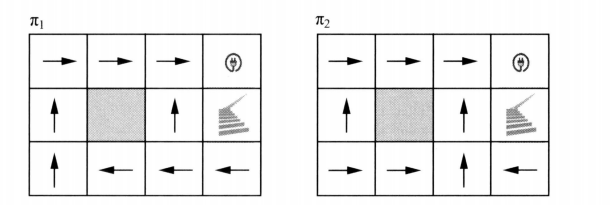
\includegraphics[width=0.8\textwidth]{img_35_6.png}
			\captionof{figure}{策略示意图}
		\end{figure}
		
		(3) 模型转换情况：
		$0.8$ 的概率会按照策略方向走，$0.1$ 的概率会向其它两个方向移动。
		若试图穿过边界则会反弹。
		
		(4) 折扣因子：
		$\gamma = 0.9$
		
		(5) 状态集合：
		$S = \{S_{11}=(1,1), S_{12}=(1,2), \dots, S_{43}=(4,3)\}$ 
		
		动作集合 $A = \{a_1(\text{向上}), a_2(\text{向右}), a_3(\text{向下}), a_4(\text{向左})\}$ 
		
		每一个状态的动作集合都是 $A$ 的子集。
		
		(6) 开始迭代：
		
		初始化：将所有格子的价值 $V(s)$ 设为 $0$，即 $V_0(s) = 0, \forall s$。
		
		利用公式：
		\[ V_{k+1}(s) = \sum_{a \in A} \pi(a|s) \left[ \sum_{s'} p(r|s,a) r + \gamma \sum_{s'} p(s'|s,a) V_k(s') \right] \]
		
		注意到此时 $r(s,a) = r(s')$，奖励仅由下一个状态决定，于是 $p(r|s,a) = p(s'|s,a)$。
		
		则：
		\[ V_{k+1}(s) = \sum_{a \in A} \pi(a|s) \cdot \sum_{s'} p(s'|s,a) (r(s') + \gamma V_k(s')) \]
		
		当 $S=S_{11}$ 时，策略是确定的 $\pi(a|S_{11}) = \begin{cases} 1 & a=a_1 \\ 0 & \text{其它} \end{cases}$。
		
		此时 $p(S_{12}|S_{11}, a_1) = 0.8$, $p(S_{21}|S_{11}, a_1) = 0.1$, $p(S_{11}|S_{11}, a_1) = 0.1$。
		
		由于 $V_k(s')=0, \forall s' \in S$，且 $r(S_{12}) = r(S_{21}) = r(S_{11}) = 0$。
		则 $V_1(S_{11}) = 0$。
		
		\vspace{0.3cm}
		
		除了 $S_{33}, S_{34}$ 之外，其余均为 $0$。下面考虑 $S_{33}$：
		$\pi(a|S_{11}) = \begin{cases} 1 & a=a_2 \\ 0 & \text{其它} \end{cases}$
		
		$p(S_{43}|S_{33}, a_2) = 0.8$, $p(S_{23}|S_{33}, a_2) = 0.1$, $p(S_{32}|S_{33}, a_2) = 0.1$。
		
		$r(S_{43}) = 1$, $r(S_{23}) = 0$, $r(S_{32}) = 0$。
		
		则 $V_1(S_{33}) = 1 \times 0.8 = 0.8$。$V_1(S_{34})$ 同理。
		
		算出第一轮结果之后，比较是否满足前后两次之差的范数是否小于阈值判断是否收敛。
		若收敛结束循环并输出，若不收敛继续循环直至收敛再输出。
		
		接下来利用 Python 求解上述过程。（代码见附录）
		\vspace{1.0cm}
		
		Python 运行结果与分析：
		
		运行结果：
		\vspace{0.5cm}
		
		% 仅花括号内的内容使用打印机字体，外部不受影响
		{
			\ttfamily
			\noindent
			======= 策略 $\pi_1$ 的状态价值 $v_{\pi1}$ ======= \\[5pt]
			\begin{tabular}{@{} l c c c c @{}} % @{} 去除表格左右边缘的额外空白
				& x= 1   & x= 2   & x= 3   & x= 4    \\
				y= 3  & 1.3616 & 1.5715 & 1.7897 &  1.0000 \\
				y= 2  & 1.1956 &  XXXX  & 1.2073 & -1.0000 \\
				y= 1  & 1.0359 & 0.9096 & 0.8391 &  0.4551 \\
			\end{tabular} \\[5pt]
			=====================================
			
			\vspace{1.0cm} % 两个表格之间的垂直间距
			
			% =====================
			% 表格 2：策略 pi2
			% =====================
			\noindent
			======= 策略 $\pi_2$ 的状态价值 $v_{\pi2}$ ======= \\[5pt]
			\begin{tabular}{@{} l c c c c @{}}
				& x= 1   & x= 2   & x= 3   & x= 4    \\
				y= 3  & 1.3616 & 1.5715 & 1.7897 &  1.0000 \\
				y= 2  & 1.1956 &  XXXX  & 1.2073 & -1.0000 \\
				y= 1  & 0.8135 & 0.8787 & 1.0008 &  0.5830 \\
			\end{tabular} \\[5pt]
			=====================================
		} % 结束打印机字体的作用域，后续内容恢复默认字体
		
		\vspace{0.5cm}
		
		结果分析：
		
		这是 Python 运行结果如上。
		其中坐标 $(1,2), (1,3), (2,3), (3,3), (3,2)$ 完全相同，这是因为两个策略在这些状态的动作都是相同的。
		而在 $(1,1), (2,1)$，$V_{\pi_1} > V_{\pi_2}$，说明此时 $\pi_1$ 的策略优于 $\pi_2$。
		在 $(3,1)$ 处 $V_{\pi_2} > V_{\pi_1}$，此时说明当下 $\pi_2$ 的策略优于 $\pi_1$。
		而 $(4,1)$ 处，虽然两个策略在此处的动作选择相同，但其结果受到 $(3,1)$ 的价值影响而导致 $V_{\pi_2} > V_{\pi_1}$。
	\end{solution}
	
	% ==========================================
	% 35.7
	% ==========================================
	\clearpage
	\begin{problem}[习题 35.7]
		图35.10 中策略逐渐收敛到 $\pi_\infty$，用策略评估算法求策略的价值函数
	\end{problem}
	
	\begin{solution}
		求解过程与题35.6类似，利用策略评估算法对求解策略$\pi_\infty$的价值函数。
		以下是策略$\pi_\infty$图：
		
		\begin{figure}[H]
			\centering
			% 【修复】这里使用了重命名后的文件 img_35_6.png
			% width=0.8\textwidth 表示图片占页面宽度的 80%
			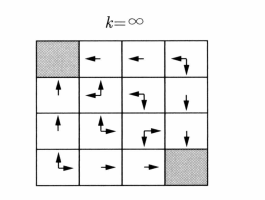
\includegraphics[width=0.4\textwidth]{img_35_7.png}
			\captionof{figure}{策略 $\pi_\infty$ 图}
		\end{figure}
		
		接下来利用 Python 求解上述过程。（代码见附录）
		
		\vspace{0.5cm}
		
		% 修复作用域：利用花括号限定打印机字体和表格间距设置
		{
			% 1. 局部使用打字机(等宽)字体
			\ttfamily 
			
			% 2. 核心调整：大幅增加列与列之间的间距 (默认是6pt，这里设为18pt以还原宽敞感)
			\setlength{\tabcolsep}{8pt}
			
			% =====================
			% 头部标题
			% =====================
			\noindent
			======= 策略 $\pi_\infty$ 的状态价值 ======= \\[3pt]
			\begin{tabular}{@{} l r r r r @{}}
				&  x=1  &  x=2  &  x=3  &  x=4  \\
				y=4   &  0.00 &  0.00 & -1.00 & -2.00 \\
				y=3   & -4.00 & -3.00 & -3.00 & -1.00 \\
				y=2   & -4.00 & -3.00 & -1.00 &  0.00 \\
				y=1   & -5.00 & -4.00 &  0.00 &  0.00 \\
			\end{tabular}
			
			\vspace{5pt}
			
			% =====================
			% 底部横线
			% =====================
			\noindent
			==================================
		}
	\end{solution}
	
	% ==========================================
	% 35.8
	% ==========================================
	\clearpage
	\begin{problem}[习题 35.8]
		例 35.1 的问题中，从起点到终点的路径规划也可以用 A* 算法求解。比较与基于 MDP 的价值迭代算法的区别，理解环境是确定和随机的意义。
	\end{problem}
	
	\begin{solution}
		A* 算法与 MDP 价值迭代算法的核心区别源于\textbf{环境建模假设}的本质不同，二者在适用场景、优化目标、求解结果与风险处理上存在显著差异，同时清晰体现了确定性环境与随机性环境的决策意义：
		
		\begin{itemize}
			\item[] \textbf{1. 环境假设与状态转移的区别}
			\begin{itemize}
				\item[] \textbf{A* 算法}：基于\textbf{确定性环境}假设，动作执行结果唯一、无随机扰动。
				执行某一移动动作（如向上），必然转移到目标相邻格点，不存在打滑、偏移等随机情况，状态转移概率为确定性的1。
				\item[] \textbf{MDP 价值迭代}：基于\textbf{随机性环境（随机状态转移）}假设，动作执行结果具有概率性。
				如本例中机器人向上移动，仅0.8概率到达目标格点，各0.1概率向两侧偏移，状态转移由概率分布描述，环境存在不可控噪声。
			\end{itemize}
			
			\item[] \textbf{2. 优化目标与评价准则的区别}
			\begin{itemize}
				\item[] \textbf{A* 算法}：以\textbf{路径代价最小}为目标，通过启发式函数（如曼哈顿距离）引导搜索，追求起点到终点的\textbf{几何最短、步数最少}的确定路径，仅考虑即时路径长度，不考虑风险与期望回报。
				\item[] \textbf{MDP 价值迭代}：以\textbf{长期折扣期望累积回报最大化}为目标，基于贝尔曼最优方程迭代更新状态价值，综合考虑转移概率、即时奖励、折扣因子，追求全局最优的期望价值，兼顾收益与随机风险。
			\end{itemize}
			
			\item[] \textbf{3. 求解输出与决策形式的区别}
			\begin{itemize}
				\item[] \textbf{A* 算法}：输出为\textbf{一条固定的最优路径序列}，是“静态的行走路线”，无法应对环境随机扰动，一旦发生偏移则原路径失效。
				\item[] \textbf{MDP 价值迭代}：输出为\textbf{全域状态的最优策略}，为每一个格点（状态）指定最优动作，是“动态的决策规则”，可应对环境随机转移带来的状态偏移，自适应调整行为。
			\end{itemize}
			
			\item[] \textbf{4. 结合例题的风险处理差异}
			\begin{itemize}
				\item[] A* 会选择紧贴楼梯（4,2）的最短路径，因不考虑随机打滑，认为无主动进入则安全；
				\item[] 价值迭代会计算偏移掉入楼梯的惩罚期望，主动选择远离陷阱的更安全路径，规避随机风险。
			\end{itemize}
			
			\item[] \textbf{5. 确定性与随机性环境的决策意义}
			确定性环境下，只需规划\textbf{唯一最优路径}即可完成任务，动作与结果一一对应；
			随机性环境下，固定路径会因转移概率失效，必须通过MDP求解\textbf{最优策略}，以期望回报为准则，在随机扰动下仍保证长期决策最优，是不确定环境下的理性决策范式。
		\end{itemize}
		
		补充A*算法对例35.1问题求解的python代码（代码见附录）。
	\end{solution}
	
	% ==========================================
	% 35.9
	% ==========================================
	\clearpage
	\begin{problem}[习题 35.9]
		例35.1的问题中，假设状态的奖励如下图所示，其他条件不变，用价值迭代算法求解各个状态的最优价值
	\end{problem}
	
	\begin{solution}
		\begin{figure}[H]
			\centering
			% 【修复】这里使用了重命名后的文件 img_35_6.png
			% width=0.8\textwidth 表示图片占页面宽度的 80%
			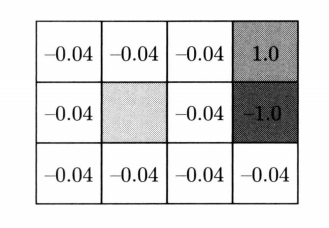
\includegraphics[width=0.4\textwidth]{img_35_9.png}
		\end{figure}
		
		价值迭代算法在求解最优价值的更新方式和策略评估的更新方式在价值函数的迭代过程不同。
		
		\begin{itemize}
			\item[] \textbf{前者（价值迭代）}是取期望回报最大的动作 $a$ 进行更新：
			\[ V_{k+1}(s) = \max_{a} \sum_{s',r} p(s',r|s,a)(r + \gamma V_k(s')) \]
			
			\item[] \textbf{后者（策略评估）}是基于当前策略 $\pi$ 的期望进行直接更新：
			\[ V_{k+1}(s) = \sum_{a} \pi(a|s) \sum_{s',r} p(s',r|s,a)(r + \gamma V_k(s')) \]
		\end{itemize}
		
		最后通过 Python 代码求出结果如下。（代码见附录）
		
		\vspace{0.5cm}
		
		\subsection*{运行结果}
		
		% 修复作用域：限制打字机字体范围
		{
			% 1. 局部使用打字机(等宽)字体
			\ttfamily 
			
			% 2. 保持宽敞的列间距，还原终端输出的视觉效果
			\setlength{\tabcolsep}{8pt}
			
			% =====================
			% 表格 1：最优价值函数 V*
			% =====================
			\noindent
			======= 最优价值函数 V* ======= \\[10pt]
			\begin{tabular}{@{} l r r r r @{}}
				&   x=1  &   x=2  &   x=3  &   x=4   \\
				y=3   & 1.2554 & 1.5106 & 1.7759 &  1.00   \\
				y=2   & 1.0535 &  XXXX  & 1.1568 & -1.00   \\
				y=1   & 0.8631 & 0.7429 & 0.9016 &  0.4650 \\
			\end{tabular}
			
			\vspace{10pt}
			\noindent
			======================================
			
			\vspace{5.0cm} % 上下两个表格的间距
			
			% =====================
			% 表格 2：最优策略 pi*
			% =====================
			\noindent
			======= 最优策略 $\pi$* ======= \\[10pt]
			% 策略表的符号（箭头、字母）通常居中对齐看起来更像图示
			\begin{tabular}{@{} l c c c c @{}} 
				&      x=1      &      x=2       &      x=3      &      x=4      \\
				y=3   & $\rightarrow$ & $\rightarrow$  & $\rightarrow$ &       T       \\
				y=2   &   $\uparrow$  & $\blacksquare$ &   $\uparrow$  &       T       \\
				y=1   &   $\uparrow$  & $\rightarrow$  &   $\uparrow$  & $\leftarrow$  \\
			\end{tabular}
			
			\vspace{10pt}
			\noindent
			============================
		}
	\end{solution}
	
	
	% ==========================================
	% 35.10
	% ==========================================
	\clearpage
	\begin{problem}[习题 35.10]
		使用价值迭代算法求例35.2中的机器人行动规划的最优价值函数和最优策略
	\end{problem}
	
	\begin{solution}
		\textbf{状态：} $\mathcal{S} = \{h (\text{高电量}), l (\text{低电量})\}$
		\textbf{动作：} $\mathcal{A} = \{w (\text{工作}), s (\text{待机}), c (\text{充电})\}$
		
		\textbf{转移概率与奖励表：}
		\begin{table}[H] % 使用 H 参数强制表格在此处
			\centering
			\begin{tabular}{ll}
				\toprule
				\textbf{转移概率} $P(s'|s,a)$ & \textbf{奖励函数} $R(s,a,s')$ \\
				\midrule
				$P(h|h,w) = 0.8$ & $R(h,w,h) = +2$ \\
				$P(l|h,w) = 0.2$ & $R(h,w,l) = 0$ \\
				$P(h|h,s) = 1.0$ & $R(h,s,h) = 0$ \\
				$P(l|l,w) = 1.0$ & $R(l,w,l) = -2$ \\
				$P(l|l,s) = 1.0$ & $R(l,s,l) = 0$ \\
				$P(h|l,c) = 1.0$ & $R(l,c,h) = +2$ \\
				\bottomrule
			\end{tabular}
		\end{table}
		
		\textbf{利用习题35.9的代码可以求解下面计算结果（代码见附录）：}
		
		\textbf{最优价值函数 V*:}
		\[
		\begin{aligned}
			V^*(h) &= 8.2759 \\
			V^*(l) &= 8.6207
		\end{aligned}
		\]
		
		\vspace{0.5cm}
		
		\textbf{最优策略 $\pi$*:}
		\[
		\begin{aligned}
			\pi^*(h) &= w \\
			\pi^*(l) &= c
		\end{aligned}
		\]
	\end{solution}
	
	% ==========================================
	% 35.11
	% ==========================================
	\clearpage
	\begin{problem}[习题 35.11]
		写出使用动作价值函数的策略评估、策略迭代和价值迭代算法
	\end{problem}
	
	\begin{solution}
		
		\begin{algorithm}[H]
			\renewcommand{\thealgocf}{} % <--- 添加这一行来隐藏算法编号
			\caption{算法 35.1（策略评估 - 动作价值）}
			\KwIn{MDP 模型、策略 $\pi$。}
			\KwOut{动作价值函数 $Q_\pi (s, a)$。}
			\KwParam{$\varepsilon > 0$。}
			
			\tcp{对所有状态-动作对的价值初始化}
			$Q(s, a) = 0$\;
			\While{$d \ge \varepsilon$}{
				\tcp{对所有状态-动作对的价值进行备份和更新}
				$U(s, a) \leftarrow Q(s, a)$\;
				$Q(s, a) \leftarrow \sum_{s', r} P(s', r | s, a) \left[ r + \gamma \sum_{a'} \pi(a'|s') U(s', a') \right]$\;
				\tcp{计算新旧价值的差异}
				$d = \max_{s, a} |U(s, a) - Q(s, a)|$\;
			}
			\Return $Q(s, a)$\;
		\end{algorithm}
		
		\vspace{1em}
		
		\begin{algorithm}[H]
			\renewcommand{\thealgocf}{} % <--- 添加这一行来隐藏算法编号
			\caption{算法 35.2（策略迭代 -动作价值）}
			\KwIn{MDP。}
			\KwOut{最优策略 $\pi_*$。}
			
			初始化策略 $\pi$\;
			\Repeat{$\pi' = \pi$}{
				使用策略评估算法求策略 $\pi$ 的动作价值函数 $Q$\;
				改进策略 $\pi$，得到新的策略 $\pi'$\;
				$\pi'(s) \leftarrow \text{argmax}_a Q(s, a), \forall s$\;
				\If{$\pi' = \pi$}{
					break\;
				}
				\Else{
					$\pi \leftarrow \pi'$\;
				}
			}
			$\pi_* = \pi'$\;
			\Return 最优策略 $\pi_*$\;
		\end{algorithm}
		
		\vspace{1em}
		
		\begin{algorithm}[H]
			\renewcommand{\thealgocf}{} % <--- 添加这一行来隐藏算法编号
			\caption{算法 35.3（价值迭代 - 动作价值）}
			\KwIn{MDP 模型。}
			\KwOut{最优动作价值函数 $Q_* (s, a)$ 及最优策略 $\pi_*$。}
			\KwParam{$\delta > 0$。}
			
			\tcp{对所有状态-动作对的价值初始化}
			$Q(s, a) = 0$\;
			\While{$d \ge \delta$}{
				\tcp{对所有状态-动作对的价值进行备份和更新}
				$U(s, a) \leftarrow Q(s, a)$\;
				$Q(s, a) \leftarrow \sum_{s', r} P(s', r | s, a) \left[ r + \gamma \max_{a'} U(s', a') \right]$\;
				\tcp{计算价值的差异}
				$d = \max_{s, a} |U(s, a) - Q(s, a)|$\;
			}
			$Q_* (s, a) \leftarrow Q(s, a)$\;
			$\pi_* \leftarrow \text{argmax}_a Q(s, a)$\;
			\Return $Q_* (s, a)$ 和 $\pi_*$\;
		\end{algorithm}
		
	\end{solution}
	
\end{document}